\documentclass[final,5p,times,twocolumn]{elsarticle}

\usepackage{graphicx}  %% For figures
\usepackage{lipsum}     %% For placeholder text
\usepackage{comment}    %% For long text comments
\usepackage{amsmath}    %% For equations
\usepackage{longtable}
\usepackage{amsmath, amssymb}
\usepackage{subcaption}
\usepackage{bbm}
\usepackage{ulem}
\usepackage{pgfplots}
\usepackage{pgfplotstable}
\pgfplotsset{compat=1.17}
\usepackage{tabularx}    % Tabelle a larghezza automatica
\usepackage{booktabs}    % Migliore stile di tabelle (toprule, midrule, bottomrule)
\usepackage{adjustbox}   % Per limitare larghezza (max width)
\usepackage[hidelinks]{hyperref}

%% Define custom commands
\newcommand{\kms}{km\,s$^{-1}$}
\newcommand{\msun}{$M_\odot$}

%% Journal name placeholder
\journal{}

\makeatletter
\def\ps@pprintTitle{%
 \let\@oddhead\@empty
 \let\@evenhead\@empty
 \let\@oddfoot\@empty
 \let\@evenfoot\@empty
}
\makeatother

\begin{document}

\begin{frontmatter}

\title{%
  \small\textsc{Università degli Studi di Salerno\\
  Corso di Laurea Magistrale in Informatica (LM-18)\\
  Intelligenza Artificiale, coorte 2025/2026 \\
  prof. Vincenzo Deufemia} \\[4pt]
  \Large Generazione Automatica di Videogiochi tramite VGDL: \\
  Un Approccio Basato su Large Language Model e Reinforcement Learning
}

%% Author information
\author{Mattia Maucioni$^1$, Antonio Landi$^1$}

\address{$^1$Track: Data Science \& Machine Learning}

\begin{abstract}
La generazione automatica di videogiochi rappresenta una sfida all'avanguardia all'intersezione tra intelligenza artificiale e generazione procedurale di contenuti. Questo lavoro indaga l'utilizzo di Large Language Model (LLM) per la generazione automatica di codice nel Video Game Description Language (VGDL), un formalismo testuale di alto livello per la descrizione di regole di gioco, interazioni tra sprite e condizioni di terminazione. Viene costruito un dataset dedicato composto da descrizioni di giochi in VGDL abbinate a corrispondenti spiegazioni in linguaggio naturale, derivate da repository open source esistenti. Vengono successivamente addestrati e valutati più LLM in tre condizioni sperimentali: inferenza zero-shot, fine-tuning supervisionato e raffinamento tramite Reinforcement Learning (RL). L'analisi comparativa tra queste condizioni consente di quantificare il contributo di ciascun paradigma di addestramento alla qualità del codice VGDL generato. Questo studio si propone di mettere in luce sia il potenziale che le attuali limitazioni degli approcci basati su LLM per la generazione formale di giochi, offrendo spunti sulle sfide legate all'applicazione dei moderni modelli linguistici a linguaggi formali specifici di dominio.
\end{abstract}


%%\begin{keyword}
%%\end{keyword}

\end{frontmatter}

\section{Introduzione}
La generazione procedurale di videogiochi è da tempo oggetto di interesse nella ricerca in intelligenza artificiale, motivata dal potenziale di automatizzare processi creativi, ridurre i costi di sviluppo e abilitare la prototipazione rapida di esperienze interattive.

Tra i formalismi proposti per rappresentare la logica di gioco in modo compatto e interpretabile, il Video Game Description Language (VGDL) \citep{6633610} si distingue come un framework particolarmente espressivo. Il VGDL consente agli sviluppatori di definire la struttura completa di un gioco attraverso una specifica testuale concisa, che comprende definizioni degli sprite, regole di interazione, mappature dei livelli e condizioni di terminazione. Questa compattezza lo rende un obiettivo naturale per i modelli generativi, poiché una descrizione VGDL semanticamente valida è sufficiente per istanziare un gioco pienamente funzionante all'interno di ambienti di simulazione compatibili come py-vgdl.

I recenti progressi nei Large Language Model hanno dimostrato capacità notevoli nei compiti di generazione di codice in un'ampia gamma di linguaggi di programmazione e formalismi specifici di dominio. Tuttavia, la loro applicazione a linguaggi altamente strutturati e semanticamente vincolati come il VGDL rimane in gran parte inesplorata. Generare codice VGDL valido a partire da descrizioni in linguaggio naturale richiede non solo correttezza sintattica, ma anche una comprensione profonda delle meccaniche di gioco, del comportamento degli sprite e della consistenza logica tra i componenti in interazione.

Questo progetto affronta tale lacuna indagando sistematicamente la capacità degli LLM di generare codice VGDL in condizioni di addestramento progressivamente più informate. A partire da un dataset costruito da repository di giochi esistenti, in cui ogni gioco è annotato con una descrizione in linguaggio naturale che ne cattura regole, obiettivi e dinamiche, vengono valutati più LLM in un contesto zero-shot per stabilire una baseline. Si applica successivamente il fine-tuning supervisionato per esporre i modelli a pattern specifici del dominio, impiegando infine tecniche di Reinforcement Learning per allineare ulteriormente gli output generati a criteri di correttezza strutturale e funzionale.

I contributi che questo lavoro si propone di raggiungere sono quattro: la costruzione di un nuovo dataset VGDL che abbina descrizioni in linguaggio naturale al corrispondente codice di gioco; una valutazione comparativa di più LLM nelle configurazioni zero-shot, supervisionata e raffinata tramite RL; un'analisi dell'efficacia del fine-tuning supervisionato e dell'RL nel migliorare la qualità funzionale delle descrizioni di gioco generate; e una discussione delle principali sfide incontrate durante l'implementazione, dalla costruzione del dataset alla progettazione della funzione di reward.

% -------------------------------------------------------
\section{Costruzione del Dataset}
% -------------------------------------------------------

La disponibilità di un dataset è un prerequisito fondamentale per addestrare e valutare LLM nel dominio specifico del VGDL. Non esistendo, a nostra conoscenza, alcun dataset pubblicamente disponibile che abbini descrizioni in linguaggio naturale a codice VGDL corrispondente, il primo contributo di questo lavoro consiste nella sua costruzione da zero.

\subsection{Raccolta dei Dati Grezzi}

Il materiale grezzo è stato raccolto principalmente dal repository ufficiale di \texttt{py-vgdl} e da raccolte derivate accessibili su GitHub, le quali includono implementazioni di giochi arcade classici (Frogger, Aliens, Zelda, ecc.) e varianti originali sviluppate dalla comunità di ricerca GVGAI. In totale sono stati estratti 201 file \texttt{.vgdl}, ciascuno composto da due blocchi principali: la game description (definizione degli sprite e delle regole di interazione) e la level description (mappatura della griglia di gioco).

Per garantire la qualità dei campioni, ogni file è stato sottoposto a un processo di rimozione del level description e validazione automatica tramite il parser interno di \texttt{py-vgdl}.

\subsection{Generazione delle Descrizioni in Linguaggio Naturale tramite LLM}

La costruzione delle annotazioni testuali ha seguito un approccio automatico basato su prompt engineering. È stato progettato un prompt strutturato che, a partire dai blocchi VGDL analizzati, istruisce il modello Claude Sonnet 4.6 (Anthropic) interrogato tramite API a generare una descrizione in linguaggio naturale del gioco articolata secondo tre dimensioni: (i) gli attori presenti nella scena e le loro proprietà cinematiche, (ii) le regole di interazione tra sprite e (iii) le condizioni di terminazione con relativo esito (vittoria o sconfitta).
Il modello ha generato iterativamente una descrizione per ciascuno dei 201 file VGDL raccolti. Le descrizioni prodotte sono state successivamente verificate per accertarne la correttezza semantica rispetto al codice sorgente corrispondente.
Il risultato è un dataset di coppie ⟨descrizione, codice VGDL⟩: la descrizione in linguaggio naturale costituisce l'input del modello e il codice VGDL corrispondente il target da generare.

\subsection{Suddivisione e Caratteristiche del Dataset}

Il dataset è stato suddiviso in 180 esempi di addestramento (\textit{train}) e 21 di test (\textit{test}). La partizione è stata eseguita in modo da garantire l'assenza di sovrapposizioni semantiche tra i due sottoinsiemi, evitando che varianti dello stesso gioco base finissero in insiemi diversi.

Il dataset consolidato e gli script di generazione, addestramento e valutazione costituiscono una pipeline riproducibile per questo dominio.

\section{Selezione dei Modelli}

La scelta dei modelli da sottoporre a valutazione ha seguito criteri che bilanciano copertura dello spazio delle architetture disponibili, accessibilità per il fine-tuning e rilevanza rispetto allo stato dell'arte nella generazione di codice.

\subsection{Criteri di Selezione}

Sono stati adottati i seguenti criteri guida nella selezione:
\begin{itemize}
  \item \textbf{Capacità di generazione di codice}: preferenza per modelli pre-addestrati su dataset che includono codice sorgente, in quanto il VGDL condivide con i linguaggi di programmazione la necessità di rispettare una sintassi formale rigida.
  \item \textbf{Dimensione del modello}: bilanciamento tra modelli di dimensione ridotta (adatti al fine-tuning su hardware accessibile) e modelli di maggiori dimensioni (utili come baseline di riferimento in modalità zero-shot).
  \item \textbf{Disponibilità dei pesi}: preferenza per modelli open-weight che consentono il fine-tuning completo o tramite tecniche efficienti quali LoRA \citep{hu2022lora}.
\end{itemize}


\subsection{Modelli Impiegati}

La fase esplorativa zero-shot ha incluso Qwen2.5-3B-Instruct \citep{qwen2.5}, Mistral-7B-Instruct-v0.3 \citep{jiang2023mistral7b}, GPT-Neo-2.7B \citep{gpt-neo} e Minerva-7B-instruct-v1.0 \citep{orlando2024minerva}. Il nucleo sperimentale, sottoposto ad adattamento supervisionato e a raffinamento con reinforcement learning, è invece costituito dai tre modelli seguenti.

\paragraph{Qwen3.5-4B} \citep{qwen3.5} Modello della famiglia Qwen da 4 miliardi di parametri, progettato per il ragionamento e la generazione di codice strutturato. Costituisce una prima baseline compatta per l'adattamento al VGDL.

\paragraph{Gemma4-E4B-it} \citep{gemma4} Modello instruction-tuned della famiglia Gemma4 di Google. È impiegato sia in modalità zero-shot tramite Ollama sia in modalità QLoRA tramite lo stack Hugging Face, consentendo di osservare direttamente l'effetto dell'adattamento supervisionato sullo stesso modello base.

\paragraph{Phi-4-mini-instruct} \citep{phi4mini} Modello instruction-tuned di Microsoft da circa 3.8 miliardi di parametri. È stato incluso come alternativa compatta ai modelli da circa 4 miliardi di parametri, per verificare se un adattamento efficiente al dominio VGDL possa compensare la minore scala del modello base.

\subsection{Protocollo di Valutazione Zero-Shot}
\label{sec:zero-shot-protocol}

I modelli sono stati valutati in modalità zero-shot sulla capacità di generare codice VGDL a partire da una descrizione in linguaggio naturale del gioco, senza alcun esempio fornito nel prompt. La valutazione si articola su due dimensioni complementari.

La prima dimensione è l'\textbf{eseguibilità} del codice generato: il VGDL prodotto dal modello viene sottoposto al parser della libreria \texttt{py-vgdl}, che ne verifica la correttezza sintattica e strutturale. Un file VGDL viene considerato valido se il parser lo accetta senza errori.

La seconda dimensione è la \textbf{similarità strutturale} con il VGDL target, ovvero il codice originale da cui è stata derivata la descrizione in linguaggio naturale fornita al modello. La similarità è calcolata dal modulo \texttt{eval\_similarity.py} tramite indice di Jaccard applicato a tre componenti estratte dal codice VGDL: gli sprite foglia definiti nel \texttt{SpriteSet} (peso 0.25), le interazioni nell'\texttt{InteractionSet} (peso 0.50) e le condizioni di terminazione nel \texttt{TerminationSet} (peso 0.25). Il punteggio finale è la media pesata dei tre indici:
\[
  \text{sim} = 0.25 \cdot J_\text{sprite} + 0.50 \cdot J_\text{interaction} + 0.25 \cdot J_\text{termination}
\]
dove $J(A, B) = |A \cap B| / |A \cup B|$. L'indice delle interazioni riceve peso doppio in quanto cattura la logica di gioco, mentre sprite e condizioni di terminazione contribuiscono in egual misura come contorno strutturale.

\section{Fine-Tuning - Learning Supervisionato}

L'approccio zero-shot fornisce una prima indicazione delle capacità generative dei modelli selezionati, ma non sfrutta la disponibilità di esempi etichettati nel dataset costruito. Il passo successivo consiste nel fine-tuning supervisionato (SFT, \textit{Supervised Fine-Tuning}): il modello viene esposto a coppie \textit{(descrizione testuale, codice VGDL target)} e aggiornato per massimizzare la verosimiglianza del codice corretto dato l'input. In questo modo il modello acquisisce familiarità con la sintassi VGDL e con le convenzioni strutturali del dominio, che difficilmente emergono dal solo pre-addestramento su dataset generici.

\subsection{Tecnologie di Training Impiegate}

Addestrare un modello da miliardi di parametri nella sua interezza richiederebbe risorse computazionali proibitive. Per questo motivo si è fatto ricorso a due tecniche complementari di efficienza.

LoRA (\textit{Low-Rank Adaptation}) è una tecnica di adattamento efficiente dei parametri (PEFT) che, anziché aggiornare l'intera matrice dei pesi, inietta coppie di matrici a basso rango $\Delta W = BA$ nei layer selezionati dell'architettura. Il numero di parametri addestrabili si riduce drasticamente: il rango $r$ controlla il compromesso tra capacità espressiva e costo computazionale.

QLoRA \citep{dettmers2023qlora} estende LoRA quantizzando il modello base a 4 bit (formato NF4, \textit{NormalFloat4}), mantenendo le matrici LoRA in precisione piena durante il forward pass. Questo permette di caricare e addestrare modelli da diversi miliardi di parametri su una singola GPU consumer, con una perdita di qualità trascurabile rispetto al full fine-tuning.

Per Qwen3.5 è stata impiegata Unsloth \citep{unsloth}, una libreria che ottimizza il training degli LLM tramite kernel CUDA e gradient checkpointing. Gemma4 e Phi-4-mini sono stati addestrati con lo stack Hugging Face, TRL e PEFT; in tutti i casi l'uso di QLoRA ha reso possibile il training su hardware consumer.

\subsection{Fine-Tuning di Qwen3.5-4B}

Il primo modello sottoposto a fine-tuning supervisionato è Qwen3.5-4B, caricato in 4-bit tramite QLoRA via Unsloth. La configurazione LoRA effettivamente salvata nell'adapter prevede rango $r=16$, $\alpha=32$ e dropout pari a $0.05$, applicata ai moduli di attenzione (\texttt{q\_proj}, \texttt{k\_proj}, \texttt{v\_proj}, \texttt{o\_proj}) e ai layer feed-forward (\texttt{gate\_proj}, \texttt{up\_proj}, \texttt{down\_proj}). Il run archiviato ha completato 3 epoche (69 step), con learning rate massimo $2 \times 10^{-4}$, scheduler cosine con 10 step di warmup, batch size effettivo pari a 8 e ottimizzatore \texttt{paged\_adamw\_8bit}. L'intera sessione si è conclusa in circa 23 minuti su singola GPU.

\begin{figure}[t]
  \centering
  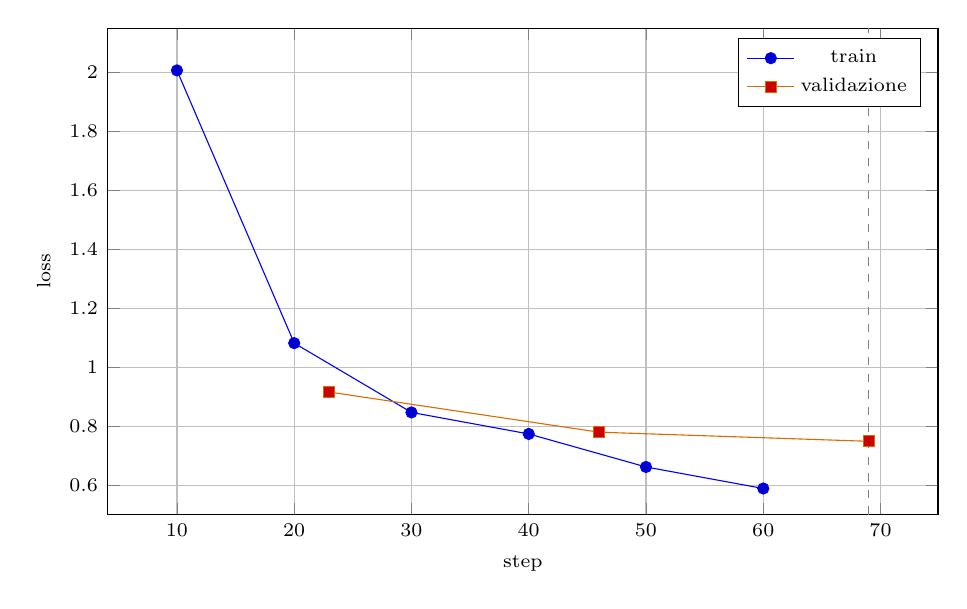
\begin{tikzpicture}
    \begin{axis}[
      width=\columnwidth, height=0.64\columnwidth,
      xlabel={step}, ylabel={loss}, ymin=0.5, ymax=2.15,
      grid=major, legend style={font=\scriptsize, at={(0.98,0.98)}, anchor=north east},
      tick label style={font=\scriptsize}, label style={font=\scriptsize}
    ]
      \addplot+[mark=*, blue] coordinates {(10,2.007) (20,1.082) (30,0.847) (40,0.774) (50,0.662) (60,0.589)};
      \addlegendentry{train}
      \addplot+[mark=square*, orange!85!black] coordinates {(23,0.916) (46,0.780) (69,0.749)};
      \addlegendentry{validazione}
      \addplot[dashed, gray] coordinates {(69,0.5) (69,2.15)};
    \end{axis}
  \end{tikzpicture}
  \caption{Curve di loss per il fine-tuning di Qwen3.5-4B, ricostruite dal log del trainer. Il miglior checkpoint è allo step 69, con validation loss $0.749$.}
  \label{fig:qwen35_loss}
\end{figure}

Come si osserva in Figura~\ref{fig:qwen35_loss}, la training loss cala rapidamente da $2.007$ a $0.589$ nell'arco delle tre epoche. La validation loss segue lo stesso andamento, da $0.916$ a $0.749$, e il checkpoint selezionato coincide con l'ultima valutazione disponibile, allo step 69. La norma del gradiente resta nell'intervallo $[0.601, 0.779]$, senza picchi anomali: il run risulta quindi numericamente stabile, ma la sua durata non consente di concludere se ulteriori epoche avrebbero portato a overfitting.

\subsection{Fine-Tuning di Gemma4-E4B-it}

Gemma4-E4B-it è stato adattato con QLoRA a 4 bit in formato NF4. L'adapter LoRA usa rango $r=16$, $\alpha=32$ e dropout $0.05$; per compatibilità con l'architettura Gemma4 l'adattamento è limitato ai moduli del language model: proiezioni di attenzione \texttt{q\_proj}, \texttt{k\_proj}, \texttt{v\_proj} e \texttt{o\_proj}, oltre ai layer MLP \texttt{gate\_proj}, \texttt{up\_proj} e \texttt{down\_proj}. In totale vengono aggiornati 34.9 milioni di parametri, pari allo $0.61\%$ dei 5.76 miliardi di parametri caricati.

Il training usa i 180 esempi di addestramento e i 21 esempi di validazione per 5 epoche, con batch per dispositivo pari a 2, gradient accumulation pari a 4, learning rate massimo $2 \times 10^{-4}$, scheduler coseno con 10 step di warmup e sequenze fino a 1024 token. Il run completa 115 step in circa 40 minuti.

\begin{figure}[t]
  \centering
  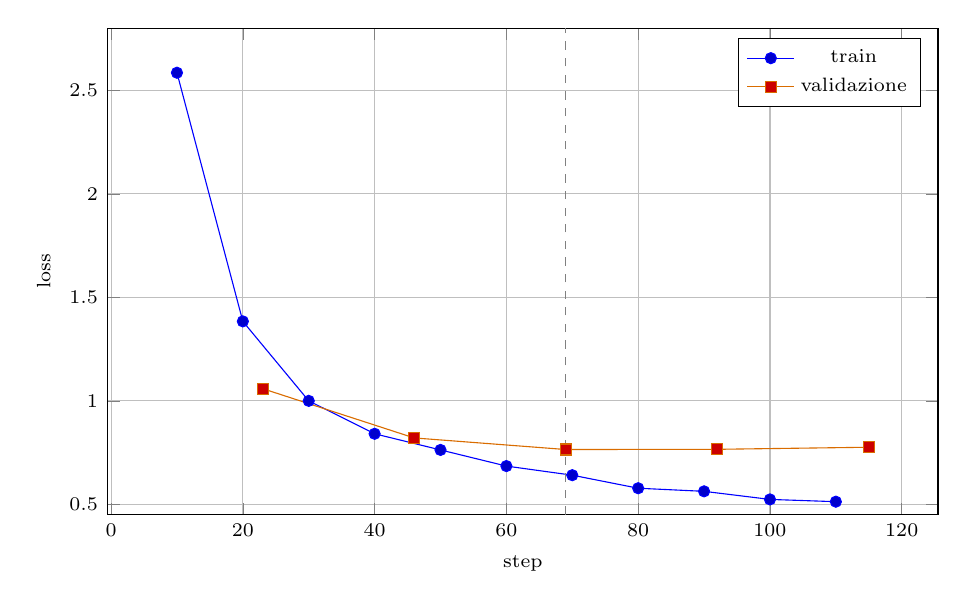
\begin{tikzpicture}
    \begin{axis}[
      width=\columnwidth, height=0.64\columnwidth,
      xlabel={step}, ylabel={loss}, ymin=0.45, ymax=2.8,
      grid=major, legend style={font=\scriptsize, at={(0.98,0.98)}, anchor=north east},
      tick label style={font=\scriptsize}, label style={font=\scriptsize}
    ]
      \addplot+[mark=*, blue] coordinates {(10,2.585) (20,1.384) (30,1.000) (40,0.841) (50,0.763) (60,0.685) (70,0.641) (80,0.578) (90,0.563) (100,0.524) (110,0.513)};
      \addlegendentry{train}
      \addplot+[mark=square*, orange!85!black] coordinates {(23,1.059) (46,0.821) (69,0.765) (92,0.766) (115,0.776)};
      \addlegendentry{validazione}
      \addplot[dashed, gray] coordinates {(69,0.45) (69,2.8)};
    \end{axis}
  \end{tikzpicture}
  \caption{Curve di loss per Gemma4-E4B-it, ricostruite dal log del trainer. Il miglior checkpoint è allo step 69, con validation loss $0.765$.}
  \label{fig:gemma4_loss}
\end{figure}

Come si osserva in Figura~\ref{fig:gemma4_loss}, la training loss cala rapidamente da $2.585$ allo step~10 a $0.513$ allo step~110. La validation loss diminuisce da $1.059$ a $0.765$ entro la terza epoca e poi cresce lievemente a $0.766$ e $0.776$. Il checkpoint selezionato è quindi quello dello step~69, con accuracy media sui token in validazione pari a $0.802$. La separazione progressiva tra training e validation loss nelle ultime epoche motiva la selezione del checkpoint intermedio, evitando di privilegiare l'ultima iterazione solo perché più aggiornata.

\subsection{Fine-Tuning di Phi-4-mini-instruct}

Il terzo modello è Phi-4-mini-instruct, addestrato con QLoRA a 4 bit tramite Hugging Face, TRL e PEFT. Anche per questo modello l'adapter salvato usa $r=16$, $\alpha=32$ e dropout $0.05$, ma i moduli adattati rispecchiano l'architettura Phi (\texttt{qkv\_proj}, \texttt{o\_proj}, \texttt{gate\_up\_proj} e \texttt{down\_proj}). Il training usa batch per dispositivo pari a 1, gradient accumulation pari a 8, sequenze fino a 2048 token e learning rate $2 \times 10^{-4}$; la loss è calcolata solo sulla completion VGDL, non sul prompt.

Per rispettare il limite di lunghezza sono stati esclusi 10 esempi di training e un esempio di test: il run ha quindi usato 169 esempi di train e 20 di validazione. Questo dettaglio è rilevante per il confronto: le loss sono utili per monitorare ogni singolo modello, ma non costituiscono una graduatoria diretta della qualità generativa fra modelli con tokenizzatori, lunghezze massime e insiemi effettivi leggermente diversi. La Tabella~\ref{tab:sft-training} riassume i risultati del training supervisionato.

\begin{table}[t]
  \centering
  \small
  \caption{Risultati dei run SFT. La validation loss è calcolata sull'hold-out interno al rispettivo run.}
  \label{tab:sft-training}
  \begin{tabular}{lccc}
    \toprule
    Modello & Train/Test & Step & Miglior loss \\
    \midrule
    Qwen3.5-4B & 180/21 & 69 & 0.749 \\
    Gemma4-E4B-it & 180/21 & 69 & 0.765 \\
    Phi-4-mini & 169/20 & 88 & 0.615 \\
    \bottomrule
  \end{tabular}
\end{table}

\begin{figure}[t]
  \centering
  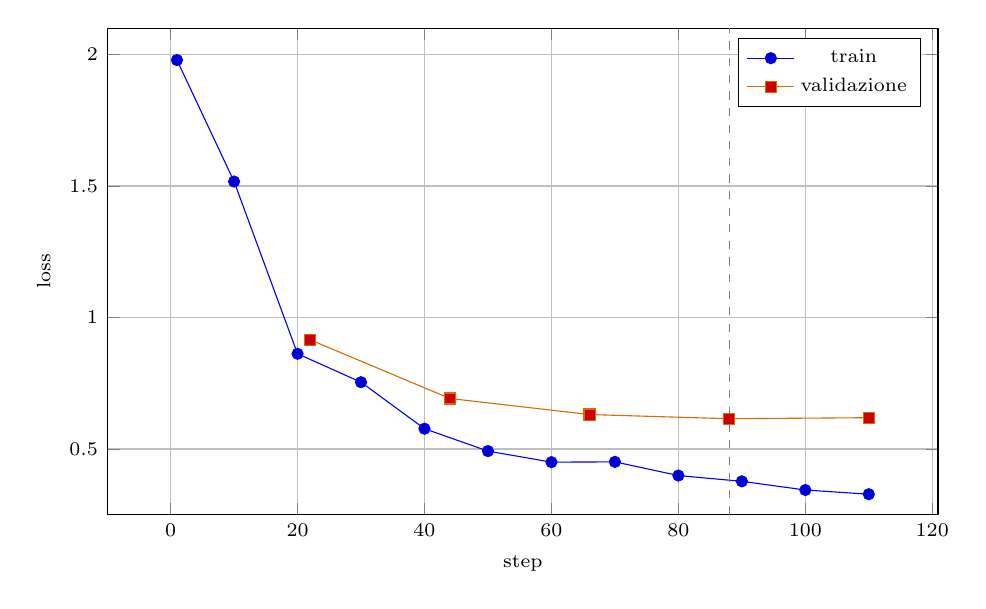
\begin{tikzpicture}
    \begin{axis}[
      width=\columnwidth, height=0.64\columnwidth,
      xlabel={step}, ylabel={loss}, ymin=0.25, ymax=2.1,
      grid=major, legend style={font=\scriptsize, at={(0.98,0.98)}, anchor=north east},
      tick label style={font=\scriptsize}, label style={font=\scriptsize}
    ]
      \addplot+[mark=*, blue] coordinates {(1,1.979) (10,1.517) (20,0.862) (30,0.754) (40,0.577) (50,0.492) (60,0.450) (70,0.451) (80,0.399) (90,0.377) (100,0.344) (110,0.328)};
      \addlegendentry{train}
      \addplot+[mark=square*, orange!85!black] coordinates {(22,0.915) (44,0.692) (66,0.631) (88,0.615) (110,0.619)};
      \addlegendentry{validazione}
      \addplot[dashed, gray] coordinates {(88,0.25) (88,2.1)};
    \end{axis}
  \end{tikzpicture}
  \caption{Curve di loss per Phi-4-mini-instruct. Il minimo di validation loss è allo step 88 (quarta epoca).}
  \label{fig:phi4_loss}
\end{figure}

Come mostra la Figura~\ref{fig:phi4_loss}, la validation loss scende da $0.915$ alla prima epoca a $0.615$ alla quarta, per poi risalire marginalmente a $0.619$ alla quinta. Il checkpoint della quarta epoca è quindi quello mantenuto per l'inferenza. La loss di training continua a diminuire fino a $0.328$, mentre il divario con la validation loss nell'ultima epoca suggerisce l'inizio di overfitting lieve. Il run ha richiesto circa 3.2 ore: un costo maggiore rispetto agli altri due esperimenti, dovuto alla lunghezza di contesto raddoppiata e alla configurazione più conservativa di batch.

\section{Reinforcement Learning con GRPO}

Il fine-tuning supervisionato insegna al modello a riprodurre le distribuzioni del dataset, ma non ottimizza direttamente i criteri operativi che rendono un VGDL utile: essere parsabile, usare l'ontologia corretta e riprodurre la struttura del gioco desiderato. Per questo è stato introdotto un secondo stadio di reinforcement learning basato su Group Relative Policy Optimization (GRPO) \citep{shao2024deepseekmath}. Per ciascuna descrizione il trainer genera $K$ completamenti, assegna una reward a ciascuno e aggiorna la policy usando vantaggi relativi al gruppo, con una penalità KL che limita l'allontanamento dalla policy iniziale. Rispetto a PPO, GRPO evita la necessità di addestrare un value model separato, caratteristica utile in un contesto con risorse hardware limitate.

\subsection{Progettazione della Reward}

La reward combina segnali sintattici e semantici e viene calcolata separatamente per ogni completamento del gruppo generato da GRPO. La funzione complessiva è
\[
R = 3r_{\mathrm{exec}} + 2r_{\mathrm{sim}} + 1.5r_{\mathrm{struct}}
    + r_{\mathrm{sprite}} + r_{\mathrm{inter}}
    + 0.5r_{\mathrm{term}} + 0.5r_{\mathrm{EOS}} + r_{\mathrm{fmt}}.
\]
Il termine $r_{\mathrm{exec}}$ assegna il massimo credito quando \texttt{py-vgdl} accetta il programma e assegna credito parziale alla presenza di \texttt{BasicGame} e delle quattro sezioni obbligatorie. $r_{\mathrm{sim}}$ è la similarità strutturale Jaccard definita nella Sezione precedente, calcolata rispetto al VGDL di riferimento. Gli altri termini verificano rispettivamente la struttura minima, classi di sprite, effetti di interazione e condizioni di terminazione ammesse dall'ontologia, l'uso di \texttt{EOS} per i bordi e l'assenza di markdown o preamboli discorsivi. Il massimo teorico è 9.5; il solo termine di formattazione può essere negativo.

Questa decomposizione fornisce un segnale denso anche alle generazioni non parsabili, ma introduce un rischio noto: un output incompleto può ottenere credito ``neutro'' per componenti assenti. Per questa ragione le metriche esterne di eseguibilità e similarità rimangono indispensabili e non vanno sostituite dalla reward di training.

\subsection{Configurazione e Risultati}

I tre esperimenti adottano lo stesso disegno della reward, ma con budget di generazione commisurati al modello. Qwen3.5 usa tre completamenti per prompt e una penalità KL con $\beta=0.01$. Gemma4 e Phi-4-mini usano due completamenti per prompt, learning rate $3\times10^{-6}$, scheduler coseno e $\beta=0.04$. Gemma4 parte dall'adapter supervisionato e usa batch per dispositivo pari a 2, gradient accumulation pari a 4, prompt fino a 512 token e completamenti fino a 384 token. La Tabella~\ref{tab:rl-config} riassume i parametri che differenziano i run.

\begin{table}[t]
  \centering
  \small
  \caption{Configurazioni GRPO dei tre modelli. $K$ indica il numero di completamenti generati per prompt.}
  \label{tab:rl-config}
  \begin{tabular}{lccc}
    \toprule
    Modello & $K$ & Max completion & $\beta$ \\
    \midrule
    Qwen3.5-4B & 3 & 384 & 0.01 \\
    Gemma4-E4B-it & 2 & 384 & 0.04 \\
    Phi-4-mini & 2 & 256 & 0.04 \\
    \bottomrule
  \end{tabular}
\end{table}

Il run Gemma4 è configurato per 3 epoche, pari a 135 step. I log fino allo step~125 mostrano una reward media compresa tra $3.56$ e $4.61$, come illustrato in Figura~\ref{fig:gemma4-grpo-reward}. Le oscillazioni sono attese: il segnale dipende da campionamenti multipli per lo stesso prompt e dalla composizione dei gruppi. Il checkpoint selezionato allo step~90 raggiunge una reward di valutazione pari a $3.902$, mentre allo step~125 la reward media di training è $4.11$. La componente di eseguibilità e quella strutturale rimangono entrambe prevalenti, coerentemente con i pesi assegnati alla sintassi e alla completezza del codice.

\begin{figure}[t]
  \centering
  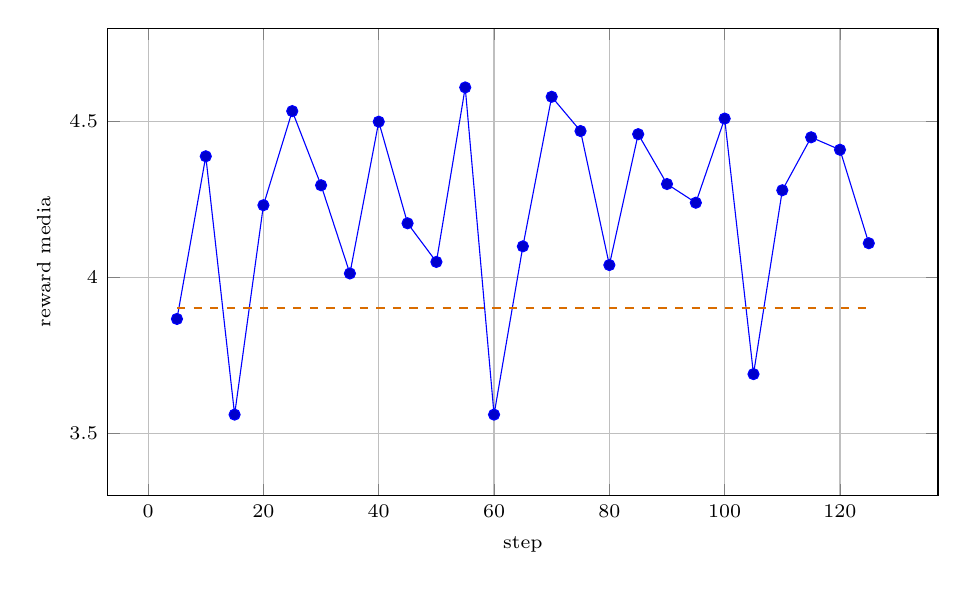
\begin{tikzpicture}
    \begin{axis}[
      width=\columnwidth, height=0.62\columnwidth,
      xlabel={step}, ylabel={reward media}, ymin=3.3, ymax=4.8,
      grid=major, tick label style={font=\scriptsize}, label style={font=\scriptsize}
    ]
      \addplot+[mark=*, blue] coordinates {(5,3.867) (10,4.389) (15,3.560) (20,4.232) (25,4.534) (30,4.296) (35,4.013) (40,4.500) (45,4.174) (50,4.050) (55,4.610) (60,3.560) (65,4.100) (70,4.580) (75,4.470) (80,4.040) (85,4.460) (90,4.300) (95,4.240) (100,4.510) (105,3.690) (110,4.280) (115,4.450) (120,4.410) (125,4.110)};
      \addplot[dashed, orange!85!black] coordinates {(5,3.902) (125,3.902)};
    \end{axis}
  \end{tikzpicture}
  \caption{Reward media durante il training GRPO di Gemma4-E4B-it. La linea tratteggiata indica la reward di valutazione del checkpoint selezionato allo step 90.}
  \label{fig:gemma4-grpo-reward}
\end{figure}

Phi-4-mini completa 3 epoche, per un totale di 135 step. La reward media oscilla tra $1.41$ e $2.27$ (Figura~\ref{fig:phi4-grpo-reward}) e la valutazione finale raggiunge $2.163/9.5$. La componente pesata di eseguibilità è $0.586$, mentre la similarità è $0.071$. Il $97.6\%$ dei completamenti di valutazione raggiunge il limite di 256 token: questo evidenzia quanto la lunghezza massima di generazione influenzi direttamente la qualità osservabile del codice VGDL.

\begin{figure}[t]
  \centering
  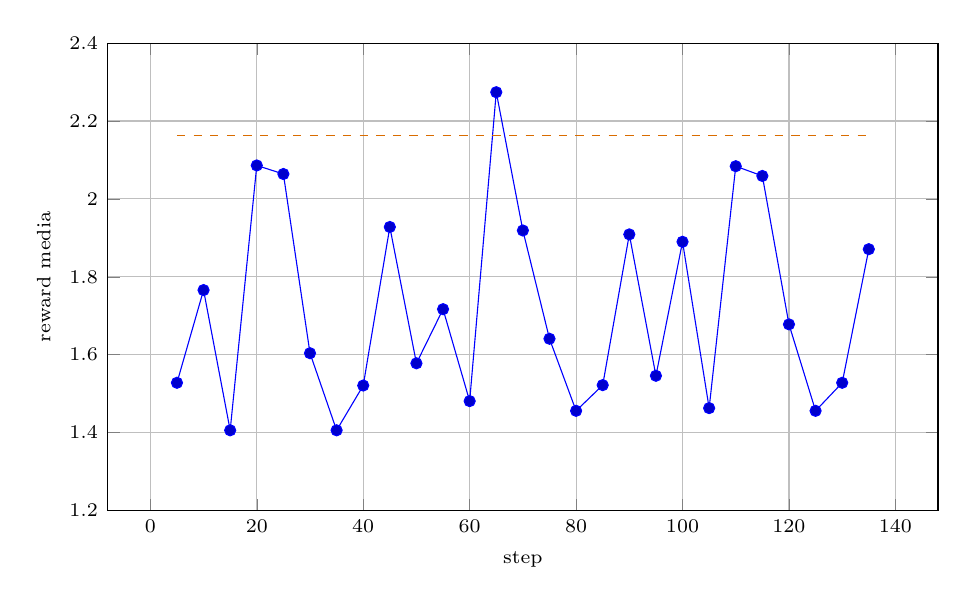
\begin{tikzpicture}
    \begin{axis}[
      width=\columnwidth, height=0.62\columnwidth,
      xlabel={step}, ylabel={reward media}, ymin=1.2, ymax=2.4,
      grid=major, tick label style={font=\scriptsize}, label style={font=\scriptsize}
    ]
      \addplot+[mark=*, blue] coordinates {(5,1.528) (10,1.766) (15,1.406) (20,2.086) (25,2.064) (30,1.604) (35,1.406) (40,1.521) (45,1.928) (50,1.578) (55,1.717) (60,1.481) (65,2.274) (70,1.919) (75,1.641) (80,1.456) (85,1.522) (90,1.909) (95,1.546) (100,1.890) (105,1.463) (110,2.084) (115,2.059) (120,1.678) (125,1.456) (130,1.528) (135,1.871)};
      \addplot[dashed, orange!85!black] coordinates {(5,2.163) (135,2.163)};
    \end{axis}
  \end{tikzpicture}
  \caption{Reward media del training GRPO di Phi-4-mini. La linea tratteggiata indica la reward media sulla valutazione finale.}
  \label{fig:phi4-grpo-reward}
\end{figure}

\section{Confronto tra Zero-Shot, SFT e GRPO}

Le valutazioni di Gemma4 sono condotte sui 21 giochi dell'hold-out, applicando le stesse procedure di eseguibilità e similarità strutturale descritte nella Sezione~\ref{sec:zero-shot-protocol}. La Tabella~\ref{tab:gemma4-test-comparison} e la Figura~\ref{fig:gemma4-test-comparison} confrontano l'inferenza zero-shot con l'adapter SFT. L'eseguibilità richiede che il parser accetti integralmente il programma; la struttura completa richiede invece la presenza di \texttt{BasicGame} e delle quattro sezioni fondamentali.

\begin{table}[t]
  \centering
  \small
  \caption{Valutazione sul test set di 21 giochi per Gemma4. Le metriche di qualità sono percentuali; il tempo è la media per generazione.}
  \label{tab:gemma4-test-comparison}
  \begin{adjustbox}{max width=\columnwidth}
  \begin{tabular}{lccccc}
    \toprule
    Condizione & Valido & Basic & Struttura & Sim. & Tempo (s) \\
    \midrule
    Zero-shot & 100.0 & 100.0 & 0.0 & 0.0 & 7.8 \\
    SFT & 0.0 & 100.0 & 85.7 & 26.1 & 107.2 \\
    \bottomrule
  \end{tabular}
  \end{adjustbox}
\end{table}

\begin{figure}[t]
  \centering
  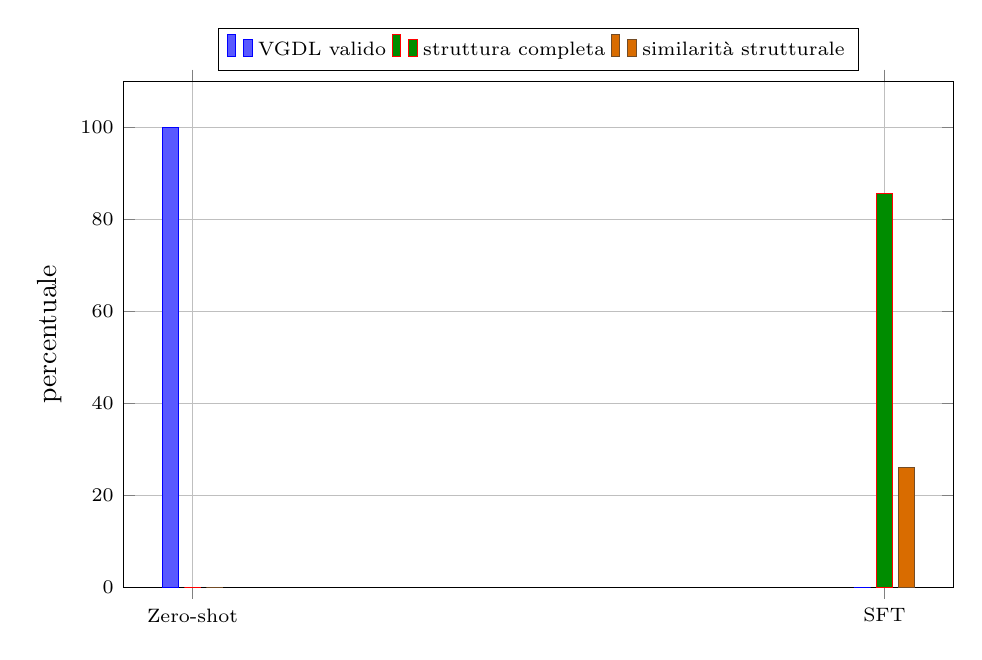
\begin{tikzpicture}
    \begin{axis}[
      ybar, width=\columnwidth, height=0.66\columnwidth,
      ylabel={percentuale}, ymin=0, ymax=110, grid=major,
      symbolic x coords={Zero-shot,SFT}, xtick=data,
      xticklabel style={font=\scriptsize}, tick label style={font=\scriptsize},
      legend style={font=\scriptsize, at={(0.5,1.02)}, anchor=south, legend columns=3},
      bar width=6pt
    ]
      \addplot+[fill=blue!65] coordinates {(Zero-shot,100.0) (SFT,0.0)};
      \addlegendentry{VGDL valido}
      \addplot+[fill=green!55!black] coordinates {(Zero-shot,0.0) (SFT,85.7)};
      \addlegendentry{struttura completa}
      \addplot+[fill=orange!85!black] coordinates {(Zero-shot,0.0) (SFT,26.1)};
      \addlegendentry{similarità strutturale}
    \end{axis}
  \end{tikzpicture}
  \caption{Confronto zero-shot e SFT di Gemma4 sull'intero test set.}
  \label{fig:gemma4-test-comparison}
\end{figure}

Il comportamento delle due condizioni è complementare. In zero-shot Gemma4 produce sempre un output accettato dal parser, ma nessuno dei programmi contiene una struttura VGDL completa o componenti in comune con il riferimento secondo la metrica Jaccard. Dopo SFT la struttura completa è presente nell'$85.7\%$ dei casi e la similarità media raggiunge il $26.1\%$: l'adapter apprende quindi le sezioni e una parte rilevante dell'ontologia specifica del dominio. L'eseguibilità scende tuttavia a zero, segnalando che la presenza delle sezioni non è sufficiente a garantire coerenza sintattica e semantica nell'intero programma.

La differenza nei tempi medi di generazione, $7.8$ s contro $107.2$ s, dipende anche dai backend impiegati: Ollama per lo zero-shot e l'inferenza Hugging Face con adapter QLoRA per SFT. Perciò il tempo è riportato come informazione operativa e non come misura diretta della qualità del modello. I valori di reward GRPO delle Figure~\ref{fig:gemma4-grpo-reward} e~\ref{fig:phi4-grpo-reward} non sono sovrapponibili alle metriche esterne della tabella: la reward è un segnale di ottimizzazione composito, mentre eseguibilità e similarità misurano una proprietà finale dell'output.

\section{Conclusioni}

Il progetto mostra che la generazione di VGDL da linguaggio naturale è affrontabile con LLM open-weight, ma che la sola plausibilità testuale non garantisce un gioco eseguibile o semanticamente vicino al riferimento. QLoRA ha consentito di adattare Qwen3.5-4B, Gemma4-E4B-it e Phi-4-mini-instruct su una GPU consumer. I tre run SFT riducono in modo consistente la validation loss; il minimo osservato è quello di Phi-4-mini ($0.615$ sul proprio hold-out), mentre Gemma4 raggiunge $0.765$ allo step~69.

La valutazione di Gemma4 sul test set evidenzia un effetto netto del SFT sulla struttura: dal $0.0\%$ di programmi completi in zero-shot all'$85.7\%$, con similarità strutturale media del $26.1\%$. Al tempo stesso, l'azzeramento dell'eseguibilità chiarisce che l'ottimizzazione della sola likelihood supervisionata non allinea automaticamente il modello al parser VGDL. Questo scarto motiva il secondo stadio GRPO, dove la validità, la struttura e la similarità entrano direttamente nel segnale di apprendimento.

I log GRPO mostrano che la reward composita guida l'ottimizzazione verso proprietà osservabili del linguaggio: Gemma4 mantiene valori elevati e seleziona un checkpoint con reward di valutazione $3.902$, mentre per Phi-4-mini il clipping quasi totale dei completamenti mette in risalto il ruolo del budget di generazione. L'infrastruttura realizzata consente quindi di analizzare separatamente correttezza formale, fedeltà strutturale e comportamento della policy, offrendo una base solida per ulteriori confronti tra zero-shot, supervisione e reinforcement learning nella generazione di giochi VGDL.

%% Bibliography
\bibliographystyle{elsarticle-num}
\bibliography{bibliografia}

\end{document}
